% @Author: AnthonyKenny98
% @Date:   2019-10-30 22:08:06
% @Last Modified by:   AnthonyKenny98
% @Last Modified time: 2020-02-23 19:11:00

% Define Document Class
\documentclass[
    11pt,           % Font Size
    letterpaper,    % Page Size
    draft,          % Draft Mode - error checking and no image rendering
    oneside         % Single Sided
]{report}           % Report Mode

% Import custom commands
\RequirePackage{../support/thesis}


%%%%%%%%%%%%%%%%%%%%%%%%%%%%%%%%%%%%%%%%%%%%%%%%%%%%%%%%%%

% DEFINE HEADER & FOOTER: (Name and Page Number)
\pagestyle{fancy}
\setlength{\headheight}{14pt}
\fancyhf{}
\rhead{Anthony JW Kenny}
\cfoot{\thepage}

% DEFINE COVER PAGE
\title{\textsc{RISC-V Architecture for Motion Planning Algorithms in Autonomous Drone Applications} \\ 
    \bigskip
    \small{A senior design project submitted in partial fulfillment of the requirements for the degree of Bachelor of Science at Harvard University} \\
\author{Anthony JW Kenny \\
        \small{S.B. Candidate in Electrical Engineering} \\ \\
        Faculty Advisor: Vijay Janapa Reddi \\ \\
        Harvard University School of Engineering and Applied Sciences \\
        \small{Cambridge, MA}}
\date{March 1st, 2020 \\ 
    \small{Version: 4.1}}}

\begin{document}

% Cover Page
\maketitle

% PREFACE
\pagenumbering{roman}
\addcontentsline{toc}{chapter}{Preface}

    % ABSTRACT
    \addcontentsline{toc}{section}{Abstract}
    % @Author: AnthonyKenny98
% @Date:   2019-10-30 22:35:34
% @Last Modified by:   AnthonyKenny98
% @Last Modified time: 2019-10-31 10:45:30

\abstract{This thesis aims to design RISC-V computer architecture that supports the fast execution of motion planning algorithms for drone applications. First, the computation of sampling-based motion planning algorithms commonly used in autonomous drones (such as \ac{RRT}, \ac{RRT*}, \ac{PRM}) will be profiled on an unmodified RISC-V processor. From this profiling, common bottlenecks and hotspots in execution will be identified. Based on these results, this project will extend the RISC-V \ac{ISA} and design a modified processor to support the extensions.}
% 78 words ^
    \clearpage

    % TABLE OF CONTENTS
    \addcontentsline{toc}{section}{Table of Contents}
    \tableofcontents
    \clearpage

    % ACRONYMNS
    \section*{List of Acronyms}
    \addcontentsline{toc}{section}{List of Acronyms}
    \input{\acronymsName}

    % ALGORITHMS
    \listofalgorithms
 
    % FIGURES
    \listoffigures

    % TABLES
    \listoftables


% CHAPTERS

% Chapter 1
\chapter{Introduction}
    \pagenumbering{arabic}                      % Change Page numbering to arabic
    % @Author: AnthonyKenny98
% @Date:   2020-02-20 00:00:23
% @Last Modified by:   AnthonyKenny98
% @Last Modified time: 2020-02-23 14:27:13



\section{Problem Summary}
    % @Author: AnthonyKenny98
% @Date:   2020-02-23 12:45:54
% @Last Modified by:   AnthonyKenny98
% @Last Modified time: 2020-02-23 14:25:32

\subsection{Background}
    \todo[inline]{TODO: Summarize the following points: \\ 
        1) Need for faster execution of motion planning in drones \\
        2) Strategy of specialized hardware \\
        3) RISC-V ISA and its potentials including extendibility \\
    }

    \subsubsection*{Robotics}
        For well over 2000 years, the concept of robotics, albeit not always with such a term, has fascinated humans. As early as the first century A.D., the Greek mathematician and engineer, Heron of Alexandria, described more than 100 different machines and automata in \textit{Pneumatica} and \textit{Automata}\cite{Alexandrinus}. In 1898, Nikola Tesla demonstrated the first radio-controlled vessel. Since then, the world has seen widespread application of robotics in manufacturing, mining, transport, exploration, and weaponry. For the last few decades, robots have operated in controlled, largely unchanging environments (e.g.\ an assembly line) where their environment and movements are largely known \textit{a priori}.
        \newline
        However, in recent years a new generation of autonomous robots has been developed for a wide range of real-world, complex applications. The increasing trend the use of autonomous robots is shown in Figure \ref{fig:useOfAutonomousRobots}. These new robots, unlike those traditional ones described above, are required to adapt to the changing environment in which they operate. As such, they must perform motion planning in real time.

        % @Author: AnthonyKenny98
% @Date:   2020-02-23 12:12:56
% @Last Modified by:   AnthonyKenny98
% @Last Modified time: 2020-02-23 13:56:51

\begin{figure}%[H]
\begin{center}
\missingfigure[figwidth=\linewidth]{Some sort of line/bar graph showing the increasing use of Autonomous robots over time. Need to find}
% 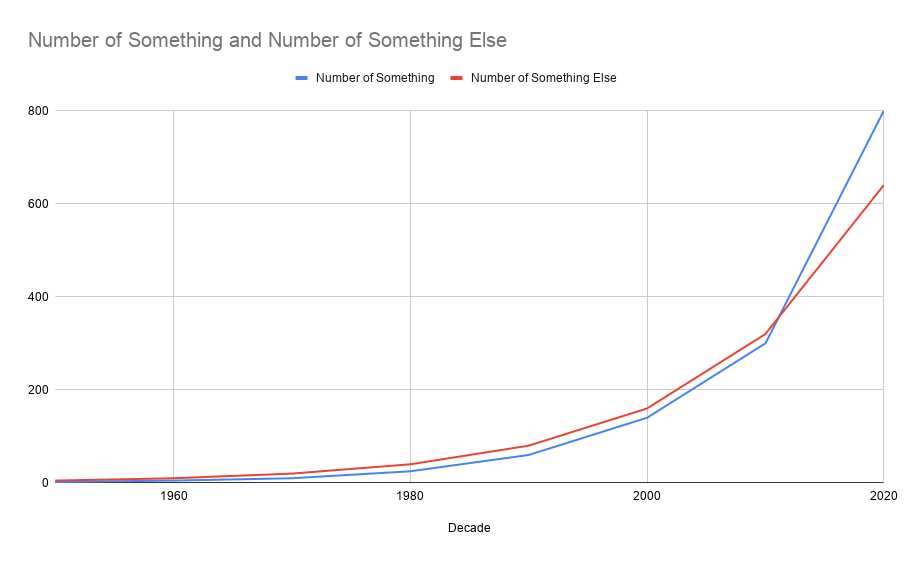
\includegraphics[width=0.8\linewidth]{img/sampleLineGraph.png}
\caption{The use of Autonomous Robots over time}
\label{fig:useOfAutonomousRobots}
\end{center}
\end{figure}

    \subsubsection*{Motion Planning}
        \todo[inline]{TODO: More of an introduction to motion planning.}
        
        Motion Planning refers to the problem of determining how a robot moves through a space to acheive a goal. Chapter \ref{chap:MotionPlanningInSoftware} provides a detailed explanation of motion planning and of \ac{RRT}, a commonly used motion planning algorithm.
        \newline
        On the algorithmic level, motion planning has been extensively studied and many solutions exist. However, current algorithms running on regular \ac{CPU}s are too slow to execute in real time for robots operating in complex environments. Simply solving this problem with more raw computing power, using energy hungry \ac{GPU}s may have merit in tethered robots. On the other hand, untethered applications, such as autonomous drones, where limiting power consumption is a primary concern, this strategy is infeasible.
        
    \subsection*{Hardware Acceleration}
        Specialized hardware designed to perform specific functions can yield significantly higher performance than software running on general purpose processors, and lower power consumption than \ac{GPU}s.
        \todo[inline]{More detail here. Reference prior work}

    \subsubsection{RISC-V}
        \todo[inline]{TODO: Introduction to RISC-V and its merits in this problem}


\subsection{Problem Definition}

    \subsubsection*{Problem Statement}
    \todo[inline]{Revise problem statement}
    Current processors cannot compute motion planning algorithms quickly enough for robots to operate in high complexity environments. Autonomous drones are a specific case of robots requiring real-time motion planning in complex environments. The state-of-the-art strategy of using a Graphics Processing Unit (GPU) to accelerate the execution of these algorithms requires too much power to be cost-effective or feasible for drones to sustain flight for useful periods of time.

    \subsubsection*{End User}
    \todo[inline]{TODO: End User}
    
\section{Prior Work}
    % @Author: AnthonyKenny98
% @Date:   2020-02-23 14:26:30
% @Last Modified by:   AnthonyKenny98
% @Last Modified time: 2020-04-05 08:02:21

\subsection{Hardware Acceleration}
    \Gls{hardware acceleration} refers to the strategy of using computer hardware specifically designed to execute a function more efficiently than can be achieved by software running on a general purpose \gls{CPU}.
    Specialized hardware designed to perform specific functions can yield significantly higher performance than software running on general purpose processors, and lower power consumption than \gls{GPU}s.

    \subsubsection*{Computer Implementation Hierarchy}
        To briefly frame the space in which this thesis operates, consider the typical computer implementation hierarchy, demonstrated in Figure \ref{fig:computerHierarchy}. \textbf{User level applications}, such as Google Chrome, Microsoft Word, and Apple's iTunes, sit at the top of the abstraction hierarchy. These applications are implemented in \textbf{High-Mid Level Languages}, such as C/C++, Python, Java, etc. These programming languages have their own hierarchy, but for the purpose of this thesis, it is sufficient to understand that these programming languages are then compiled into \textbf{Assembly Language}. Assembly language closely follows the execution of instructions on the \textbf{processor}, and is defined by an \textbf{\gls{ISA}}. An \gls{ISA} can be thought of as the contract between software programmers and processor engineers, agreeing what instructions the processor is able to implement. This assembly code is finally loaded into the processor's instruction memory and executed. 
        % @Author: AnthonyKenny98
% @Date:   2020-02-29 23:52:30
% @Last Modified by:   AnthonyKenny98
% @Last Modified time: 2020-04-10 12:37:43
\begin{figure}[H]
\begin{center}
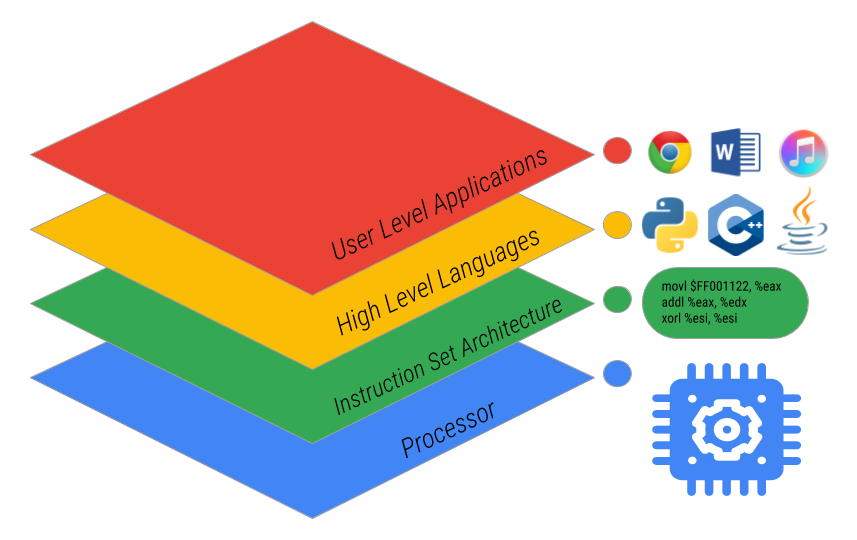
\includegraphics[width=\linewidth]{chapters/chapter1/img/computerHierarchy.png}
\mycaption{Simple Visualization of Computer Implementation Hierarchy}{}
\label{fig:computerHierarchy}
\end{center}
\end{figure}
        As will be outlined in Section \ref{section:projectOverview}, this thesis operates extensively on the lower two levels of this hierarchy, extending an existing \gls{ISA} and building hardware at the processor level that supports these extensions.

    \subsubsection*{Acceleration of Motion Planning}
        Accelerating motion planning with hardware is a fairly well studied problem. \\
        \textit{A Motion Planning Processor on Reconfigurable Hardware} \cite{Atay2006} studied the performance benefits of using \gls{FPGA}-based motion planning hardware as either a motion planning processor, co-processor, or collision detection chip. It targeted the feasibility checks of motion planning (largely collision detection) and found their solution could build a roadmap using the \gls{PRM} algorithm up to 25 times faster than a Pentium-4 3Ghz CPU could. \\
        In \textit{A Programmable Architecture for Robot Motion Planning Acceleration} \cite{Murray}, Murray et al. built on the work of the aformentioned paper, to accelerate several aspects of motion planning in an efficent manner. \\
        \textit{FPGA based Combinatorial Architecture for Parallelizing RRT} \cite{Malik2015} studies the possibility of building architecture to allow multiple \gls{RRT}s to work simultaneously to uniformly explore a map. Taking advantage of hardware parallelism allows systems such as this to compute more information per clock cycle. \\
        Finally, in the paper \textit{Robot Motion Planning on a Chip} \cite{Murrayb}, Murray et al. describe a method for contructing robot-specific hardware for motion planning, based on the method of constructing collision detection circuits for \gls{PRM} that are completely parallelised, such that edge collision computation performance is independent of the number of edges in the graph. With this method, they could compute motion plans for a 6-degree-of-freedom robot more than 3 orders of magnitude faster than previous methods.

    \subsection{RISC-V}
    \subsubsection{Extending RISC-V}
    RISC-V is designed cleverly in a modular way, with a set of base instruction sets and a set of standard extensions. As a result, processors can be designed to only implement the instruction groups it requires, saving time, space and power on instructions that won't be used. In addition, another goal of RISC-V is to provide a basis for more specialized instruction-set extensions or more customized accelerators. This is described in the most recent \textit{RISC-V Instruction Set Manual} \cite{Waterman2019}. This is a powerful feature, as it does not break any software compatability, but allows for designers to easily follow the steps outlined in Figure \ref{fig:extendingRISCV}. From a \gls{hardware acceleration} point of view, this is particularly useful as it allows the designer to directly invoke whatever functional unit or accelerator they implement from assembly code.
    % @Author: AnthonyKenny98
% @Date:   2020-03-01 10:28:34
% @Last Modified by:   AnthonyKenny98
% @Last Modified time: 2020-03-01 10:32:45
\begin{figure}[H]
\begin{center}
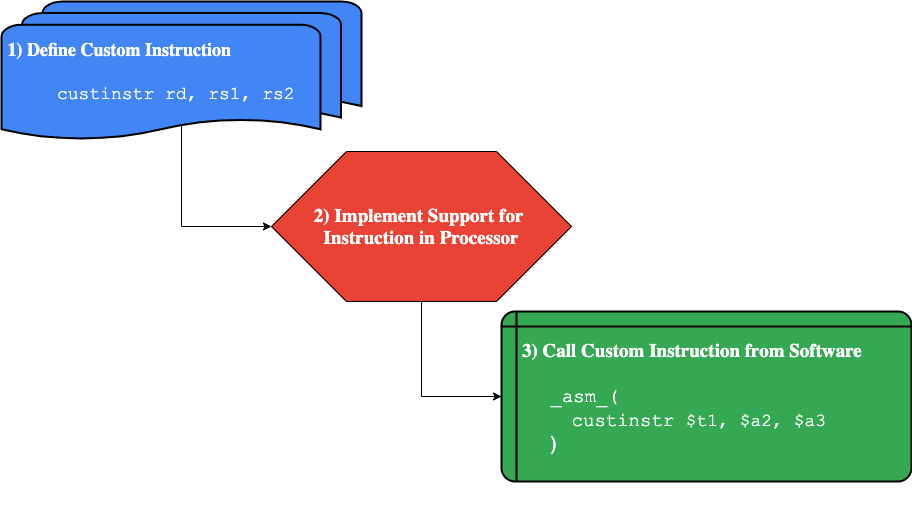
\includegraphics[width=0.9\linewidth]{chapters/chapter1/img/extendingRISCV.png}
\caption{Typical Process of Adding Non-Standard Extension to RISC-V ISA}
\label{fig:extendingRISCV}
\end{center}
\end{figure}

    \subsubsection{Accelerating RISC-V Processors}
    Having only been released in 2011, RISC-V is still a relatively unexplored opportunity for non-education applications. However, it shows promise in the commercial space, with Alibaba recently developing the Xuantie, a 16-core, 2.5GHz processor, currently the fastest RISC-V processor. Recently there has been promising research into accelerating computationally complex applications, particularly in edge-computing, with RISC-V architecture. \\
    \textit{Towards Deep Learning using TensorFlow Lite on RISC-V}, a paper co-written by the faculty advisor of this thesis, V.J. Reddi, presented the software infrastructure for optimizing the execution of neural network calculations by extending the RISC-V ISA and adding processor support for such extensions. A small number of instruction extensions achieved coverage over a wide variety of speech and vision application deep neural networks. Reddi et al. were able to achieve an 8 times speedup over a baseline implementation when using the extended instruction set.
    \textit{GAP-8: A RISC-V SoC for AI at the Edge of the IoT} proposed a programmable RISC-V computing engine with 8-core and convolutional neural network accelerator for power efficient, battery operated, IoT edge-device computing with order-of-magnitude performance improvements with greater energy efficiency. \\



\section{Project Overview}
    % @Author: AnthonyKenny98
% @Date:   2020-02-23 14:27:21
% @Last Modified by:   AnthonyKenny98
% @Last Modified time: 2020-02-23 14:28:10

\subsection{Proposed Solution}
    \todo[inline]{Proposed Solution}


\subsection{Project Specifications}
    \todo[inline]{Project Specifications}

\subsection{Project Structure}
    \todo[inline]{Project Structure/Timeline}



\newpage

    \lhead{Chapter \thechapter}                 % Include Chapter name on subsequent headers


% Chapter 2
\chapter{Motion Planning in Software}
    \label{chap:MotionPlanningInSoftware}
    % @Author: AnthonyKenny98
% @Date:   2020-02-22 15:42:12
% @Last Modified by:   AnthonyKenny98
% @Last Modified time: 2020-04-05 17:17:11

The first objective of this thesis is to identify a typical motion planning algorithm, profile its execution, and determine computational bottlenecks.\todo{Update once I have properly defined goals and objectives}

This chapter introduces the concept of motion planning and details the process of implementing and analysing \glsfirst{RRT}, a commonly used algorithm, to identify its computational bottlenecks.\\

\section{Motion Planning Background} 
\label{section:motion_planning_background}
    % @Author: AnthonyKenny98
% @Date:   2020-04-04 10:01:40
% @Last Modified by:   AnthonyKenny98
% @Last Modified time: 2020-04-05 10:56:20

A funny paradox in computer science is the fact that it is relatively easy to teach a computer to perform tasks that humans find very complicated, but extremely difficult to program one to execute functions that humans master during infancy. Consider, it was as early as 1949 that Claude Shannon presented his paper \textit{Programming a Computer for Playing Chess}\cite{Shannon1950}, and by 1997 the \textit{Deep Blue} computer defeated Garry Kasparov, reigning world champion, in a six game chess match.\cite{Campbell2002} Compare that with some of the most advanced autonomous humanoid robots to date displaying dexterity only comparable with that of a toddler. The task of finding a collision free path, performed constantly without thought by a human, is an example of this paradigm. For a robot to compute a collision free path, it relies on a set of Motion Planning Algorithms.

Motion Planning Algorithms refer to the set of algorithms that find possible sequences of valid \gls{configuration}s for a robot in a space. In plain English, they are algorithms that determine the movements a robot can make in a map, with the intent of eventually finding a path from one point to another. 

\subsection{Key Concepts}
    \subsubsection{\Gls{workspace}}
    The \gls{workspace}, more loosely known as the \textbf{map}, is the space which the robot and obstacles occupy. Obviously, \textbf{obstacles} refer to anything with which the robot cannot intersect.
    
    \subsubsection{Configuration}
    A configuration describes the position, orientation, and pose of the robot. The complexity of a robot's configuration is therefore dependant on the dimension of the \gls{workspace}, the complexity of the robot itself, and in what level of detail the robot must be represented. For example:
    \begin{itemize}
        \item Most simply, a robot can be represented as a point by the Cartesian coordinates $(x,y)$ \gls{2D} space and $(x,y,z)$ in \gls{3D} space.
        \item More realistically, a robot such as a drone may be represented in \gls{3D} by an origin point $(x,y,z)$ and 3 Euler angles $(\alpha,\beta,\gamma)$ describing its orientation.
        \item In a more complex form, a fixed base robot with $N$ \glsfirst{DOF} would require an $N$-dimensional configuration.
    \end{itemize}

    % @Author: AnthonyKenny98
% @Date:   2020-04-04 11:13:58
% @Last Modified by:   AnthonyKenny98
% @Last Modified time: 2020-04-04 12:09:59
% @Author: AnthonyKenny98
% @Date:   2020-02-29 17:30:44
% @Last Modified by:   AnthonyKenny98
% @Last Modified time: 2020-04-03 14:28:30
\begin{figure}[H]
\begin{center}
\begin{tabular}{cc}

    % Subfigure A
    \begin{subfigure}{0.4\textwidth}
    \begin{center}
    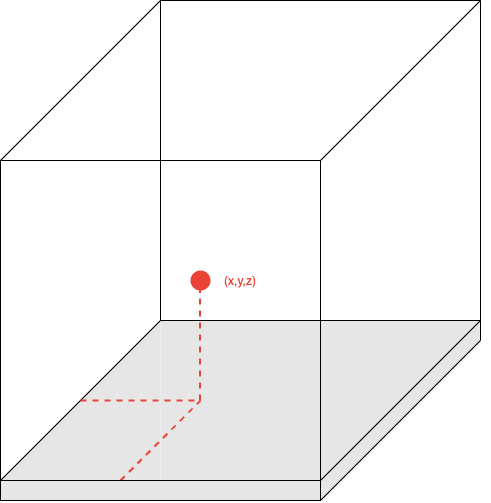
\includegraphics[width=\linewidth]{chapters/chapter2/img/motionPlanning/3DPointConfiguration.png}
    \caption{A robot represented by just a point in 3D space, requiring only 3 Cartesian coordinate $(x,y,z)$ points to describe its \gls{configuration}}
    \label{subfig:3DPointConfig}
    \end{center}
    \end{subfigure}
    &
    % 
    % Subfigure B
    \begin{subfigure}{0.4\textwidth}
    \begin{center}
    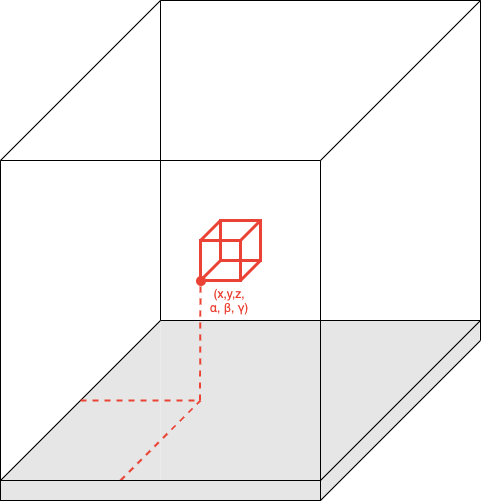
\includegraphics[width=\linewidth]{chapters/chapter2/img/motionPlanning/3DCubeConfiguration.png}
    \caption{A robot represented as a cube in 3D space, now requiring 3 Euler angles $(\alpha, \beta, \gamma)$ along with the original Cartesian coordinates.}
    \label{subfig:3DCubeConfig}
    \end{center}
    \end{subfigure} \\
\end{tabular}
    % Caption and Label
    \caption{Example of 2 Robot Configurations in 3D Space for Motion Planning Purposes}
    \label{fig:configuration}

\end{center}
\end{figure}

    \subsubsection{Occupancy Grid Map}
    An \glsfirst{OGM} is a method of representing the obstacles present in a \gls{workspace}. Obstacles are often irregularly shaped and computing collisions with such obstacles is near impossible. Therefore, the \gls{workspace} is discretized into grids and grids containing any part of the obstacle are markes as occupied, even if only a small part of the grid is occupied. An \gls{OGM} will more accurately represent a \gls{workspace} with a higher resolution, shown in Figure \ref{fig:OGM}.

    % @Author: AnthonyKenny98
% @Date:   2020-04-04 12:27:50
% @Last Modified by:   AnthonyKenny98
% @Last Modified time: 2020-04-06 15:13:14
% @Author: AnthonyKenny98
% @Date:   2020-04-04 11:13:58
% @Last Modified by:   AnthonyKenny98
% @Last Modified time: 2020-04-04 12:09:59
% @Author: AnthonyKenny98
% @Date:   2020-02-29 17:30:44
% @Last Modified by:   AnthonyKenny98
% @Last Modified time: 2020-04-03 14:28:30
\begin{figure}[H]
\begin{center}
\begin{tabular}{cc}

    % Subfigure A
    \begin{subfigure}{0.4\textwidth}
    \begin{center}
    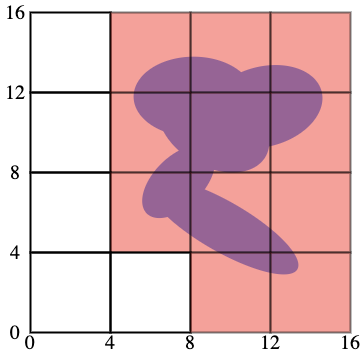
\includegraphics[width=\linewidth]{chapters/chapter2/img/motionPlanning/OGMlowres.png}
    \caption{}
    \label{subfig:OGM_A}
    \end{center}
    \end{subfigure}
    &
    % 
    % Subfigure B
    \begin{subfigure}{0.4\textwidth}
    \begin{center}
    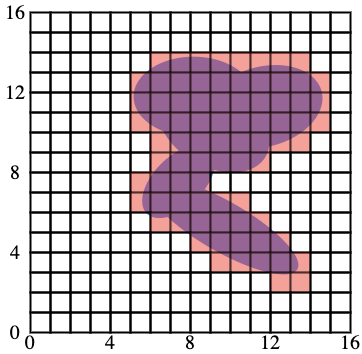
\includegraphics[width=\linewidth]{chapters/chapter2/img/motionPlanning/OGMhighres.png}
    \caption{}
    \label{subfig:OGM_B}
    \end{center}
    \end{subfigure} \\
\end{tabular}
    % Caption and Label
    \mycaption{Occupancy Grid Maps for a (16$\times$16) Workspace of Different Resolutions}{. Figure \ref{subfig:OGM_A} shows how an OGM with low resolution, while simpler to construct and analyse, will over-represent the obstacle density of a workspace. Figure \ref{subfig:OGM_B} shows how a higher resolution will more accurately reflect the obstacles of a workspace.}
    \label{fig:OGM}

\end{center}
\end{figure}

\subsection{Algorithms}
    
    \subsubsection{Scope}
    \todo[inline,caption=Finish Scope]{Part of the problem, it is not about sensing obstacles, building map, or finding shortest path. It is merely about exploring the space and building a tree of possible paths}

\todo[inline]{Finish this Section, should describe why I chose RRT}


\newpage
\section{Implementation of RRT}
\label{section:rrt}
    % @Author: AnthonyKenny98
% @Date:   2020-02-22 15:53:59
% @Last Modified by:   AnthonyKenny98
% @Last Modified time: 2020-04-05 13:31:53

% INTRO
\glsfirst{RRT} is an algorithm designed to efficiently build a tree of collision-free paths in a high-complexity environment. The algorithm randomly samples points, draws an edge from the nearest currently existing node in the tree, to grow the tree in the space. It is inherently biased to grow towards large unsearched areas of the workspace. RRT was developed by S. LaVelle\cite{LaValle1998} and J. Kuffner\cite{LaValle2001}. It is used in autonomous robotic motion planning problems such as autonomous drones.

% ALGORITHM
\subsection{Algorithm}

    % SCOPE OF ALGORITHM
    \subsubsection{Scope}
        \gls{RRT} takes an \glsfirst{OGM} as its input. This \gls{OGM} may be built and updated using \gls{a priori} knowledge, sensor data from the robot, and other inputs. \gls{RRT} will output a tree of collision free paths toward the goal, as demonstrated in Figure \ref{fig:rrt_scope}. \textbf{It does not calculate the fastest path from that tree}; that can be accomplished using algorithms such as \Gls{dijkstra's algorithm}.

        % @Author: AnthonyKenny98
% @Date:   2020-04-05 10:54:20
% @Last Modified by:   AnthonyKenny98
% @Last Modified time: 2020-04-05 11:05:47

\begin{figure}[H]
\begin{centering}
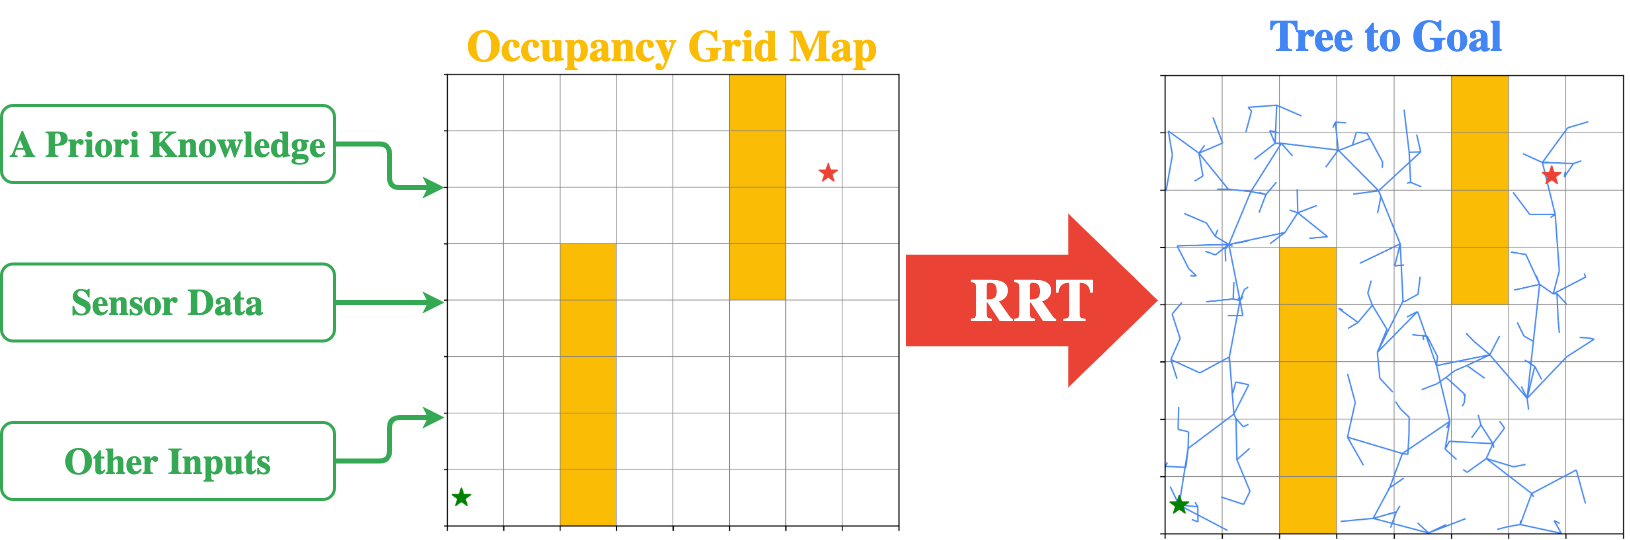
\includegraphics[width=\linewidth]{chapters/chapter2/img/RRT-Scope.png}
\caption[Scope of the RRT Algorithm]{Scope of the RRT Algorithm: Takes an \gls{OGM} as input and outputs a tree of collision free paths through that \gls{OGM}. The tree is shown in blue on the right.} 
\label{fig:rrt_scope}
\end{centering}
\end{figure}

    % BASIC RRT - BUILDING THE TREE
    \subsubsection{Building the Tree}

        Put simply, \gls{RRT} finds a path from start to finish by randomly exploring a workspace.
        Put more technically, it builds a tree of possible \glspl{configuration} (also known as a graph), connected by edges, for a robot of some physical description. It does so by selecting random \glspl{configuration} and adding them to the graph. 
        From this graph, a path from the initial \gls{configuration} to some goal \gls{configuration} can be found, given a high enough number of iterations. As such, \gls{RRT} can be considered \gls{probabilistically complete}.
        The pseudo-code for \gls{RRT} can be seen in Algorithm \ref{algorithm:rrt}
        
        % RRT Algorithm
        % @Author: AnthonyKenny98
% @Date:   2020-02-27 10:55:29
% @Last Modified by:   AnthonyKenny98
% @Last Modified time: 2020-02-27 15:45:23

\begin{algorithm}[H]
    \caption{Rapidly-Exploring Random Tree in Free Configuration Space}
    \SetAlgoLined
    \SetArgSty{textnormal}
    \begin{tabular}{l l}
    \textbf{Inputs:}    & Initial configuration $q_{init}$,\\ 
                        & Number of nodes in graph $K$, \\
                        & Incremental Distance $\Delta q$ \\
    \textbf{Output:}    & RRT Graph $G$ with $K$ configurations \& edges \\
    \end{tabular}

        $G$.init()\;
        \For{$k = 1$ to $K$}{
            $q_{rand} \leftarrow $ randomConfiguration(); \\
            $q_{near} \leftarrow $ nearestVertex($q_{rand}$, $G$); \\
            $q_{new} \leftarrow $ newVertex($q_{near}$, $q_{rand}$, $\Delta q$); \\
            $G$.addVertex($q_{new}$); \\  
            $G$.addEdge($q_{near}$, $q_{new}$);
        }
\label{algorithm:rrt}
\end{algorithm}

        % Explanation of Algorithm, referencing visual step by step figure
        Algorithm \ref{algorithm:rrt} can be visually represented in Figure \ref{fig:rrt-step-by-step}. Consider a \gls{2D} robot operating in a \gls{2D} workspace. A Graph $G$ is initialized containing an initial \gls{configuration}, $q_{init}$, with constraints on the number of nodes that the graph can hold, $K$, and the maximum distance between two nodes, $\Delta q$. This is shown in Sub-figure \ref{subfig:rrt-step-by-step-A}. A random \gls{configuration} for the robot, $q_{rand}$ is generated (\ref{subfig:rrt-step-by-step-B}). The nearest existing \gls{configuration} in $G$, $q_{near}$, is found. (In the first iteration, $q_{near} = q_{init}$, shown in Sub-figure \ref{subfig:rrt-step-by-step-C}). The distance between $q_{near}$ and $q_{rand}$ is calculated. If this distance is less than $\Delta q$, $q_{new} = q_{rand}$. If not, $q_{new}$ is selected, typically by moving by $\Delta q$ from $q_{near}$ towards $q_{rand}$ (\ref{subfig:rrt-step-by-step-C}). $q_{new}$ is then added to $G$. This is repeated for $K$ \gls{configuration}s.
        \todo[inline]{This is all really ugly and should be explained better}

        % Step By Step RRT Figure
        % @Author: AnthonyKenny98
% @Date:   2020-02-27 14:22:10
% @Last Modified by:   AnthonyKenny98
% @Last Modified time: 2020-02-27 15:36:30

\begin{figure}[H]
\begin{center}
\begin{tabular}{c c}

    % Subfigure A
    \begin{subfigure}{0.45\textwidth}
    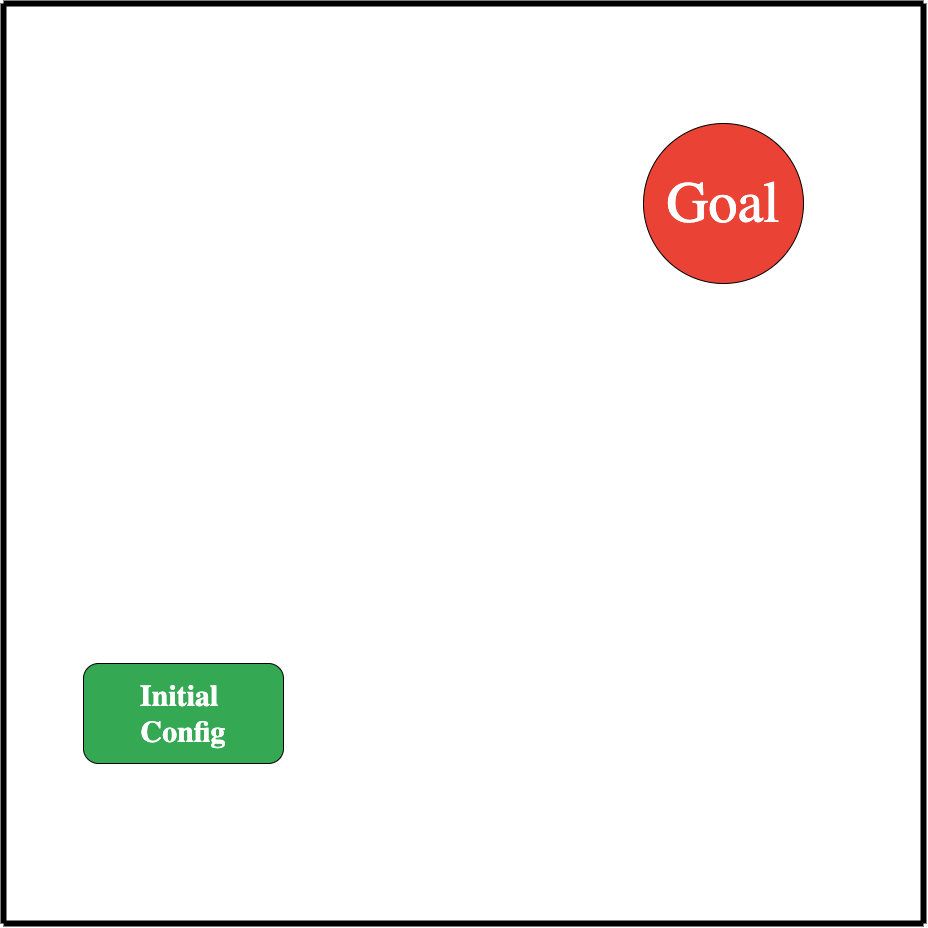
\includegraphics[draft=false,width=\linewidth]{chapters/chapter2/img/RRT_step_by_step-A.png}
    \caption{Graph $G$ contains only $q_{init}$ \newline}
    \label{subfig:rrt-step-by-step-A}
    \end{subfigure} &
    % 
    % Subfigure B
    \begin{subfigure}{0.45\textwidth}
    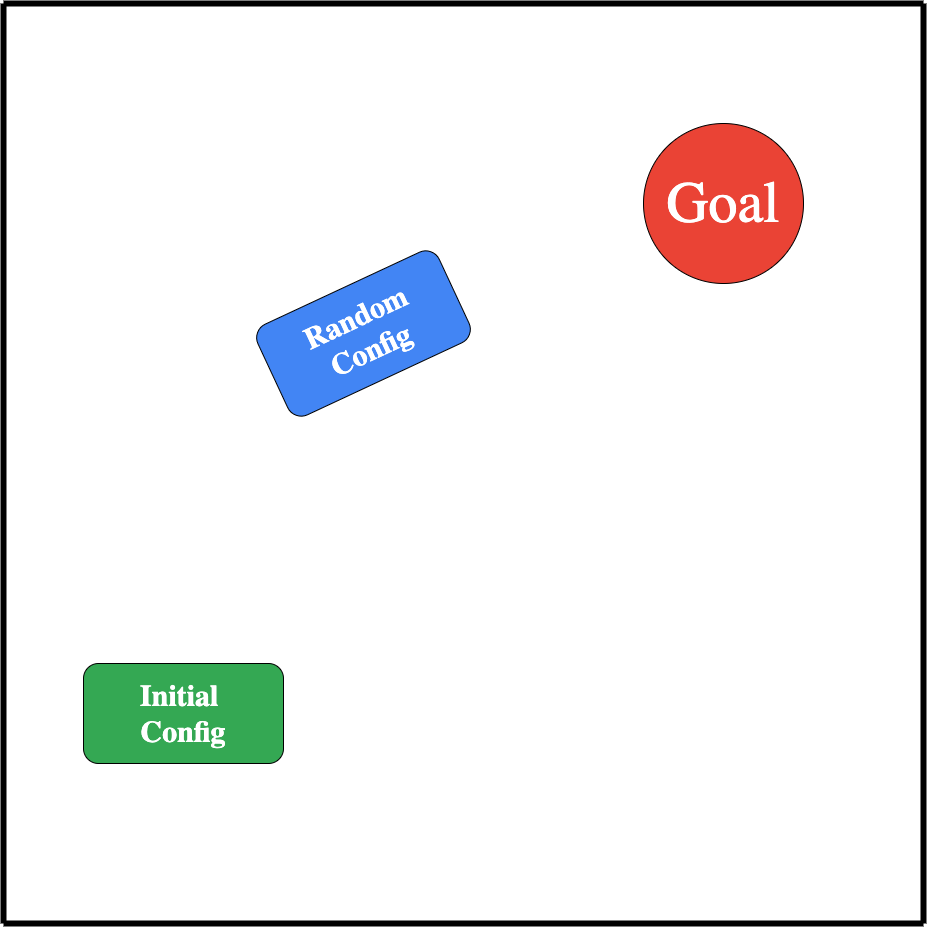
\includegraphics[draft=false,width=\linewidth]{chapters/chapter2/img/RRT_step_by_step-B.png}
    \caption{The first random configuration, $q_{rand}$, is generated}
    \label{subfig:rrt-step-by-step-B}
    \end{subfigure} \\ \\

    % Subfigure C
    \begin{subfigure}{0.45\textwidth}
    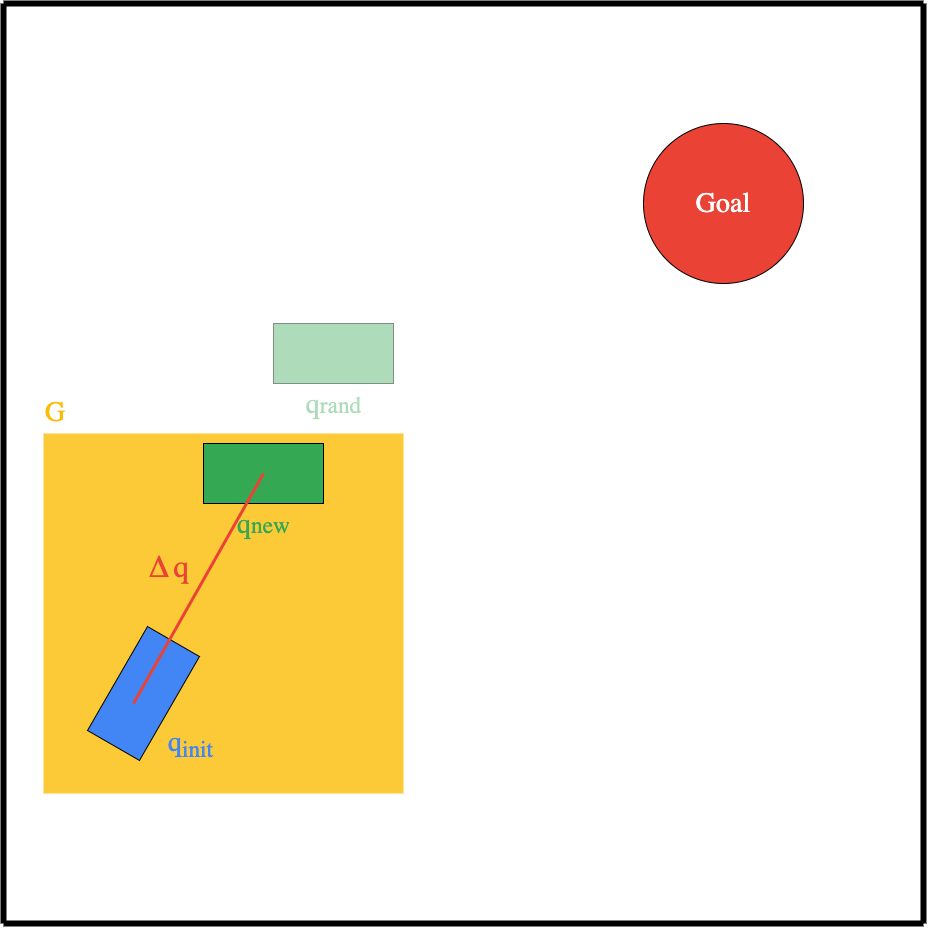
\includegraphics[draft=false,width=\linewidth]{chapters/chapter2/img/RRT_step_by_step-C.png}
    \caption{In first iteration, $q_{near} = q_{init}$. Distance between $q_{init}$ and $q_{rand}$ is greater than $\Delta q$, so $q_{new}$ is generated and added to $G$}
    \label{subfig:rrt-step-by-step-C}
    \end{subfigure} &
    % 
    % Subfigure D
    \begin{subfigure}{0.45\textwidth}
    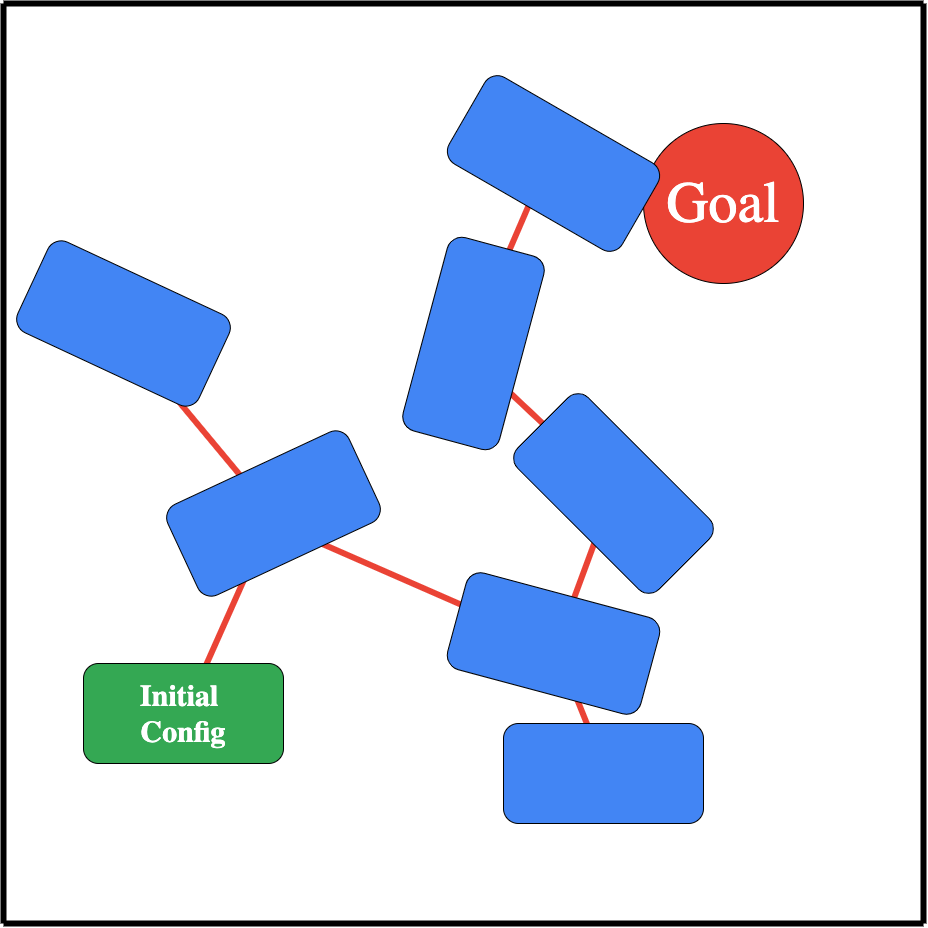
\includegraphics[draft=false,width=\linewidth]{chapters/chapter2/img/RRT_step_by_step-D.png}
    \caption{This is repeated $K$ times. For $G$, $K=10$, and the red line represents the edges between configurations}
    \label{subfig:rrt-step-by-step-D}
    \end{subfigure}

\end{tabular}
    
    % Caption and Label
    \caption{Step by step demonstration of \ac{RRT} Algorithm for 2D robot in 2D space}
    \label{fig:rrt-step-by-step}
\end{center}
\end{figure}
        \todo{Redo this diagram}

    % COLLISION DETECTION
    \subsubsection{Collision Detection}

        Algorithm \ref{algorithm:rrt} shows how \gls{RRT} builds a graph of possible \gls{configuration}s connected by edges in a completely free \gls{configuration} space. However, in real-world applications, a robot's \gls{workspace} space often contains obstacles. As such, collision detection must be included in the algorithm. The two types of collisions the algorithm must check for are \textit{configuration collisions} (those where the robot would collide with an obstacle in a given \gls{configuration}) and \textit{edge collisions} (where the robot would collide when moving between two collision free \gls{configuration}s).

        The RRT with \gls{configuration} and edge collision detection can be seen in Algorithm \ref{algorithm:rrt_collision}. The method of implementing \gls{RRT} with collision detection to model a drone in 3D space is detailed in Section \ref{section:implementation}.

        % @Author: AnthonyKenny98
% @Date:   2020-02-27 18:27:36
% @Last Modified by:   AnthonyKenny98
% @Last Modified time: 2020-04-03 14:28:31
\bigskip
\begin{algorithm}[H]
    \caption{Rapidly-Exploring Random Tree with Collision Detection}
    \SetAlgoLined
    \SetArgSty{textnormal}
    \begin{tabular}{l l}
    \textbf{Inputs:}    & Initial \gls{configuration} $q_{init}$,\\ 
                        & Number of nodes in graph $K$, \\
                        & Incremental Distance $\Delta q$, \\
                        & Space $S$ containing obstacles \\
    \textbf{Output:}    & RRT Graph $G$ with $K$ \gls{configuration}s $[q]$ \& edges $[e]$ \\
    \end{tabular}

        $G$.init()\;
        \For{$k = 1$ to $K$}{
            \While { !\text{pointCollision}($q_{new}$) } {
                $q_{rand} \leftarrow $ randomConfiguration(); \\
                $q_{near} \leftarrow $ nearestVertex($q_{rand}$, $G$); \\
                $q_{new} \leftarrow $ newVertex($q_{near}$, $q_{rand}$, $\Delta q$); \\
            }
            $e_{new} \leftarrow $ newEdge($q_{near}, q_{new}$) \\
            \eIf{\text{!edgeCollision($e_{new}$)}} {
                $G$.addVertex($q_{new}$); \\  
                $G$.addEdge($q_{near}$, $q_{new}$);
            }{
                $k = k-1$;
            }
        }
\label{algorithm:rrt_collision}
\end{algorithm}
\bigskip

\newpage

% IMPLEMENTATION OF RRT
\subsection{Implementation}\label{section:implementation}
    
    % TECHNICAL SPECIFICATIONS
    \subsubsection{Technical Specifications}

        With \gls{RRT} selected as the benchmark algorithm against which to test specialised hardware, this project required an implementation of the algorithm that satisfied the following criteria.\todo{Better RRT Implementation introductory sentence}

        % Tech Spec Table
        \begin{table}[H]
\begin{center}
\begin{tabular}{|p{.3\linewidth}|p{.64\linewidth}|}
    \hline
    Requirement             & Description and Justification \\
    \hline
    C/C++ Implementation    & As outlined in Section \ref{subsection:project_structure}, the critical step in determining the design of specialized hardware to accelerate \ac{RRT} is CPU performance analysis of the algorithm to determine computational hot-spots. Implementations in C allow for the use of certain CPU profiling tools, described in Section \ref{subsubsection:vtune}, unlike higher-level languages such as Python. \\
    \hline
    Models Drone as Point   & In reality, implementing \ac{RRT} for a drone would model the robot as a \ac{3D} object defined by coordinates $\{x, y, z\}$ and Euler angles $\{\alpha, \beta, \gamma \}$. However, for simplicity's sake, modelling the drone as a point defined by coordinates $\{x, y, z\}$ will suffice. Time permitting, this could be revisited. \todo[inline]{Change this based on whether time does permit} \\
    \hline
    Mirrors Algorithm       & In order for the results of CPU performance analysis to be easy to understand, software implementation of \ac{RRT} should call functions that mirror the functions described in Algorithms \ref{algorithm:rrt} and \ref{algorithm:rrt_collision}. \\
    \hline
\end{tabular}
\caption{Technical Specifications for \ac{RRT} Implementation}
\label{table:RRT_Tech_Specs}
\end{center}
\end{table}
\todo[inline]{Improve this table}

        The original intention was to find an existing implementation of RRT that could fulfill these requirements. Most open source implementations found online were in Python, and all those implemented in C were unsuitable, as they had extraneous \gls{GUI}s, reliance on external \gls{API}s, and other features that would distort analysis of algorithmic hot-spots. Appendix \ref{section:rrt_appendix_existing_implementations} is shows an evaluation of existing implementations.\cite{RoboJackets2019}\cite{Planning2019}\cite{Sourishg2017}\cite{Vss2sn2019}.

        As a result, it was necessary to build a C implementation of RRT from the ground up that satisfied the requirements in Table \ref{table:RRT_Tech_Specs}. It can be found in this project's GitHub repository. It follows Algorithm \ref{algorithm:rrt_collision} closely. For monitoring correctness, I build in an optional \gls{GUI} that shows the tree, starting node, and obstacles.

    \subsubsection*{Modelling a \gls{UAV} for RRT}

    \subsubsection{Implementation in 2D}
    The first step was to implement RRT with a 2-Dimensional workspace. \todo[inline]{More detail}
    % @Author: AnthonyKenny98
% @Date:   2020-02-23 14:14:12
% @Last Modified by:   AnthonyKenny98
% @Last Modified time: 2020-03-01 08:06:12


\begin{figure}[H]
\begin{center}
\begin{tabular}{c  c}
    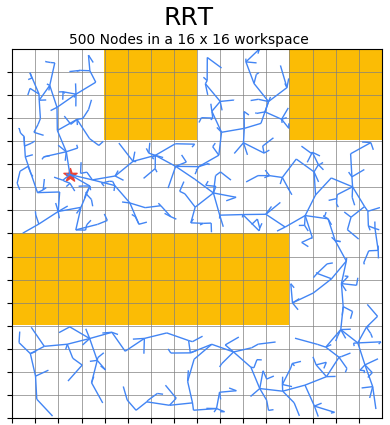
\includegraphics[width=0.45\linewidth]{chapters/chapter2/img/rrt_2d_1.png} & 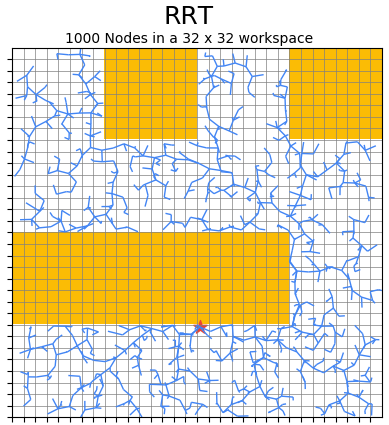
\includegraphics[width=0.45\linewidth]{chapters/chapter2/img/rrt_2d_2.png} \\
    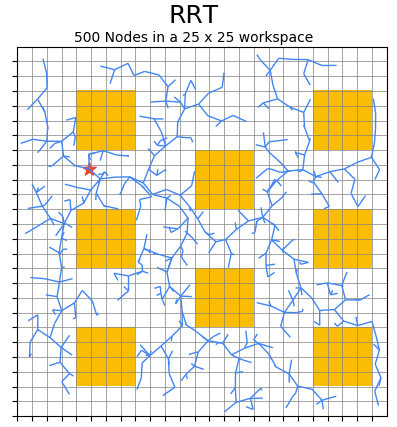
\includegraphics[width=0.45\linewidth]{chapters/chapter2/img/rrt_2d_3.png} & 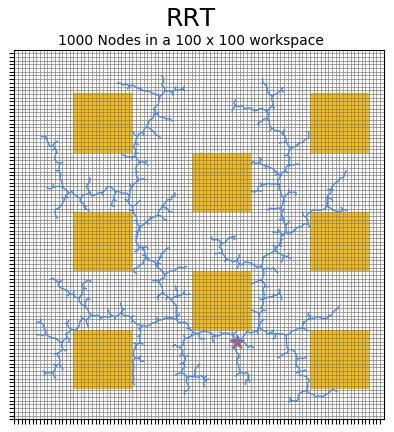
\includegraphics[width=0.45\linewidth]{chapters/chapter2/img/rrt_2d_4.png}
    \end{tabular}
    \caption{2D RRT Implementation shown by \ac{GUI}}
    \label{figure:2DrrtGui}
\end{center}
\end{figure}

    \subsubsection{Implementation in 3D}
    \todo[inline]{Describe implementation in 3D}
    % @Author: AnthonyKenny98
% @Date:   2020-02-23 14:14:12
% @Last Modified by:   AnthonyKenny98
% @Last Modified time: 2020-03-01 13:51:49


\begin{figure}[H]
\begin{center}
    \begin{tabular}{c  c}
    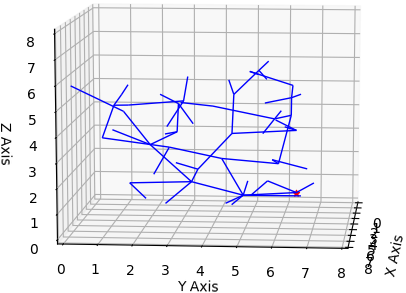
\includegraphics[width=0.45\linewidth]{chapters/chapter2/img/rrt_3d_1.png} & 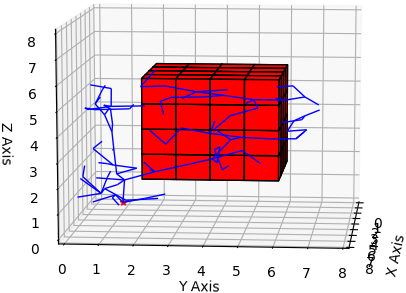
\includegraphics[width=0.45\linewidth]{chapters/chapter2/img/rrt_3d_2.png} \\
    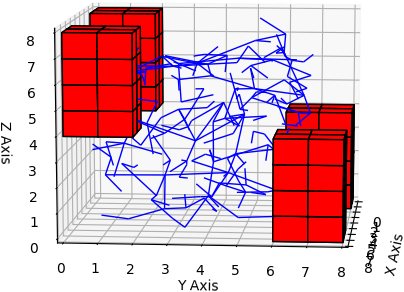
\includegraphics[width=0.45\linewidth]{chapters/chapter2/img/rrt_3d_3.png} & 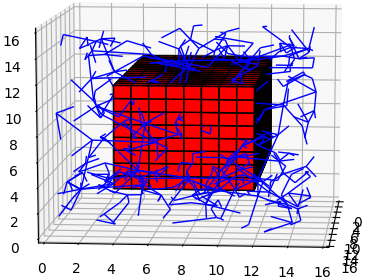
\includegraphics[width=0.45\linewidth]{chapters/chapter2/img/rrt_3d_4.png}
    \end{tabular}
    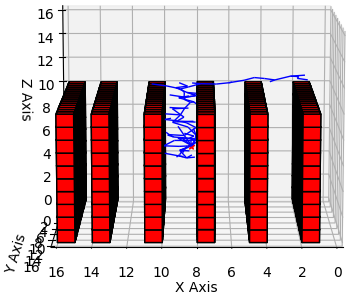
\includegraphics[width=0.45\linewidth]{chapters/chapter2/img/rrt_3d_5.png}
    \caption{3D RRT Implementation shown by \ac{GUI}}
    \label{figure:3DrrtGui}
\end{center}
\end{figure}


\newpage
\section{Analysis of RRT}
\label{section:rrt_analysis}
    % @Author: AnthonyKenny98
% @Date:   2020-02-28 15:02:19
% @Last Modified by:   AnthonyKenny98
% @Last Modified time: 2020-02-28 23:28:59

\todo[inline]{Brief introduction outlining purpose of performance analysis}

\subsection{Methodology}
    To restate, the aim of this thesis is to design a computer processor with reduced execution time of motion planning algorithms, such as \ac{RRT}. As such, it is important to understand the elements of the algorithm that have the highest percentage of CPU execution time. To determine this, it was necessary to implement my own, naive but typical, \ac{RRT} in C. This program could then be compiled and analysed using a software performance profiling tool. With this, I could design experiments to determine the critical RRT functions (those occupying a majority of CPU time) and see how this varies given different parameters.
    \todo[inline]{Outline of method of analysis. Something better than the above}

    \subsubsection{VTune Profiler}
    \label{subsubsection:vtune}
        VTune Profiler performance profiler is an application for software performance analysis. It provides functionality to examine hot-spots for CPU execution time through a top down analysis, shown below in Figure \ref{figure:VTuneTopDown}. As can be seen from the figure, the top down analysis tool shows the percentage of CPU time taken up by each function. I used this tool to profile the algorithm's performance as I changed certain parameters.
        \todo[inline]{Rewrite the above}
        % @Author: AnthonyKenny98
% @Date:   2020-02-23 14:33:19
% @Last Modified by:   AnthonyKenny98
% @Last Modified time: 2020-02-23 14:36:06

\begin{figure}[H]
\begin{center}
    \missingfigure[figwidth=\linewidth]{Screenshot of VTune Top Down Analysis (Maybe)}
    \caption{VTune Amplifier TopDown Analysis Example}
    \label{figure:VTuneTopDown}
\end{center}
\end{figure}

    \subsubsection{Internal Timing}
        The limitation of VTune Profiler is that it can only profile software running on Intel processors, which implement the x86-64 \ac{ISA}. As such, when the time comes to analyse performance of the software running on a RISC-V processor, another method will be required. A simple and effective way of measuring execution performance is to insert timing functionality into the software itself. 

    \subsubsection{Comparison}

\subsection{Results}
\label{section:rrt_analysis_results}

% Chapter 3
\chapter{Motion Planning in Hardware}

% Chapter 4
\chapter{RISC-V Processor}

% Chapter 5
\chapter{Discussion}

% Conclusion
\chapter{Conclusion}

\bibliography{\bibliographyName}
\bibliographystyle{ieeetr}

\begin{appendices}

\chapter{Project Repository}
    \label{appendix:repository}
    % @Author: AnthonyKenny98
% @Date:   2020-02-23 14:22:13
% @Last Modified by:   AnthonyKenny98
% @Last Modified time: 2020-02-23 14:23:03

\todo[inline]{TODO: Provide information about this project's repository}
\ifdraft{
        \chapter{General ToDos}
        \begin{enumerate}
            \item Use glossary package
            \item Use better acronym package that includes plurals
        \end{enumerate}
}

\end{appendices}
\clearpage



\end{document}  
